%bonus slides

% 13. data rates +
% 14. KCDC +
% 15. ML/DL opportunities +
% 16. GRADLC initiative +
\begin{frame}
 \huge
 \center
 Bonus slides
\end{frame}


%GRADLC initiative descripton 

\begin{frame}{German-Russian Astroparticle \\Data Life Cycle Initiative\footnotemark[1]}
\vspace{-1.4em}
\begin{center}
  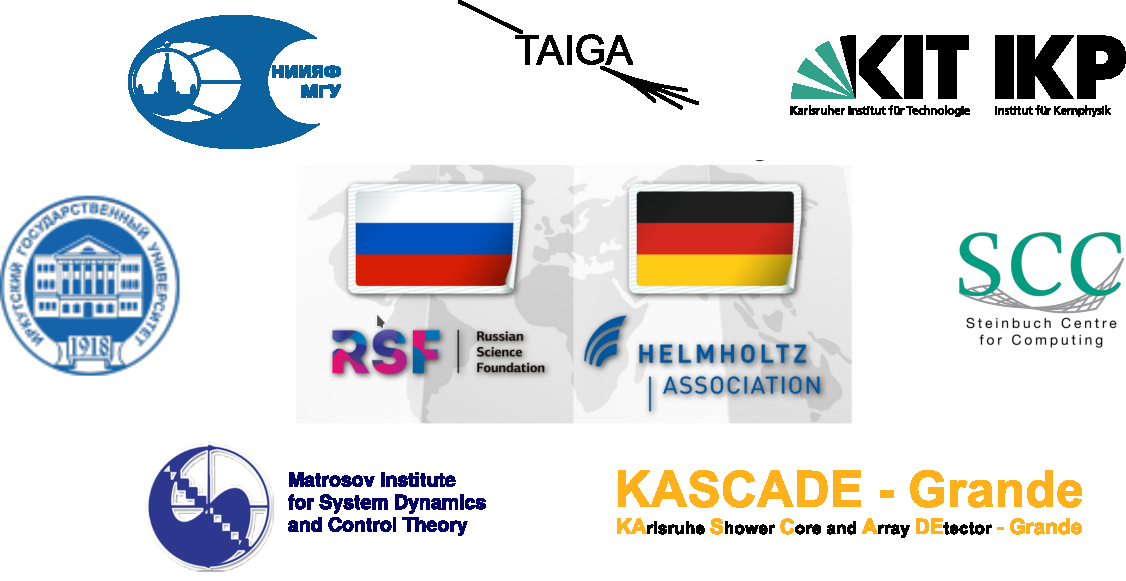
\includegraphics[width=0.9\textwidth]{pics/Collab-4.pdf}
\end{center}
\footnotesize\footnotetext[1]{Granted by RSF-Helmholtz Joint Research Groups}
\end{frame}

% %experiments overview

\begin{frame}{KASCADE-Grande}
\begin{itemize}
  \item Proposed in 1989---disassembled in 2013;
  \item Aimed at studying
  high-evergy (galactic) cosmic rays by observing extensive air showers (EAS);
%   processes at the edge of the Galaxy and beyond by observing extended atmospheric showers (EAS);
  \item Consisted of:
  \begin{itemize}
    \item scintillator arrays:
%     detecting $e$, $\gamma$, $\mu$:
    \begin{itemize}
  %сцинтиляторы, различают e, gamma, mu
    \item KASCADE---256 stations;
    \item GRANDE---37 stations;
    \end{itemize}
 %один большой калориметр
    \item Hadronic callorimeter;
 %радиодетектор
    \item Digital radio array LOPES;
%     detecting $e$, $e^{+}$;
% позволяющих наблюдать различные компоненты ливня
  \end{itemize}
  \item Important features of cosmic-ray spectrum have been obtained. The data analysis is ongoing;
%  благодаря данным с эксперимента было открыто много всего ополезного, при этом анлиз данных продолжается. новые статьи выходят
  \item KCDC (\textbf{K}ASCADE \textbf{C}osmic Ray \textbf{D}ata \textbf{C}enter, \textcolor{blue}{\texttt{http://kcdc.ikp.kit.edu}}) is a dedicated portal where all the data collected are available online. % At the moment
\end{itemize}

\begin{tikzpicture}[remember picture,overlay]
  \node[xshift=-12ex,yshift=-21ex] at (current page.north east){%
    
\includegraphics[width=0.3\textwidth]{pics/KCDC-Logo.png}
  };
\end{tikzpicture}
% \parbox[t][0pt]{0pt}{
%   \vspace{-0.63\textheight}
%   ~\hspace{0.68\textwidth}
\includegraphics[width=0.3\textwidth]{pics/KCDC-Logo.png}
% }
\end{frame}

\begin{frame}{TAIGA - Tunka Advanced Instrument for cosmic ray physics and Gamma Astronomy}
% \footnotesize
% % \vspace{-1em}
\begin{itemize}
 \item The detectors construction started in 90s with Tunka-25 setup;
 \item Changed name from Tunka to TAIGA;
 \item Is ongoing and continiously enhancend;
%  \item Currently consists of 4 detectors presented + TUNKA IACT is under construction;
\end{itemize}

% \vspace{2em}

\begin{center}
    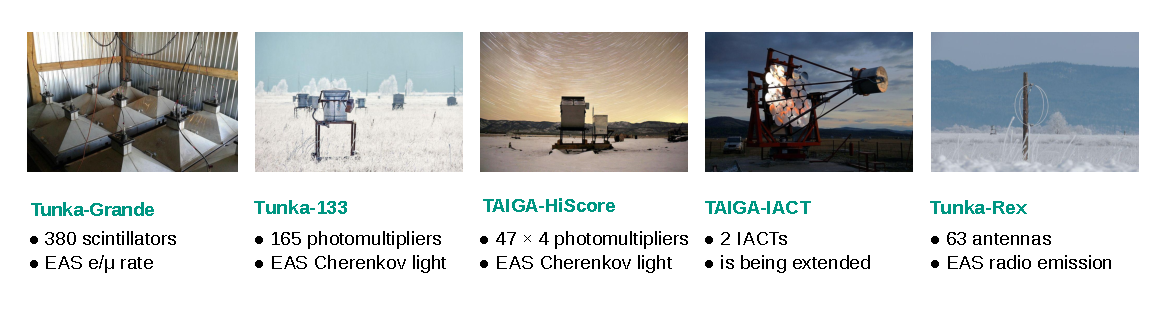
\includegraphics[width=1\textwidth]{pics/TAIGA_exp_wt.pdf} 
\end{center}

\end{frame}

 - experiments overview. Is not requiered is this IT=specified presentation
% 
% \begin{frame}{The main objectives}
% \begin{minipage}[c]{0.45\textwidth}
%   \begin{itemize}
%     \item  Provide sustainable access to scientific data
%     \item  Archiving of Data and Metadata
%     \item  Providing analysis tools
%     \item  Education in Big Data Science
%   \end{itemize}
% \end{minipage}
% \hfill
% \begin{minipage}[c]{0.54\textwidth}
%   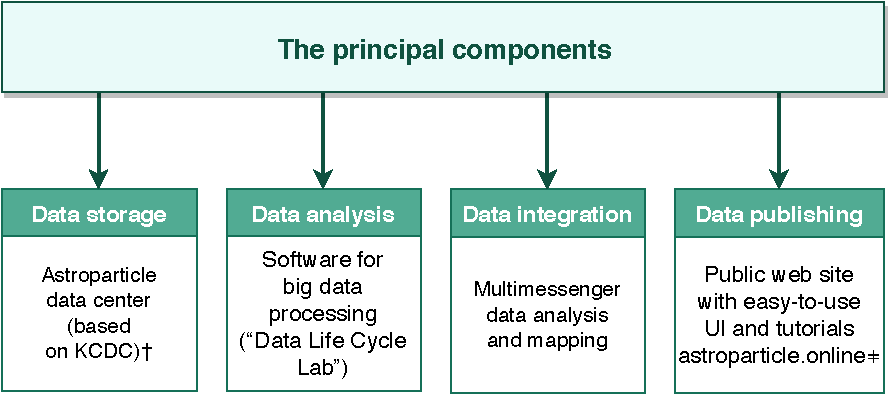
\includegraphics[width=1\textwidth]{pics/proj_objectives.pdf}
% \end{minipage}
%   \vspace{-\topsep}
%   \vspace{-\partopsep}
%   \vspace{\itemsep}
%   \vspace{\parsep}
%   \begin{itemize}
%     \item  Development area for multi-messenger analyses (e.g. Deep Learning)
%     \item  Platform for communication and exchange within Astroparticle Physics
%   \end{itemize}
% \end{frame}
% 


\begin{frame}{KASCADE Cosmic-ray Data Center (KCDC)}
    \begin{itemize}
        \small
        \setlength{\itemsep}{0pt}
        \item providing free, unlimited, reliable open access to KASCADE cosmic ray data at \textcolor{blue}{\underline{https://kcdc.ikp.kit.edu}};
        \item almost all KASCADE data is available;
        \item selection of fully calibrated quantities and detector signals;
        \item information platform: physics and experiment backgrounds, tutorials, meta information for data analysis;
        \item archive of KASCADE software and data;
        \item uses modern and open source web technologies.
    \end{itemize}


\includegraphics[height=0.35\textheight]{pics/KCDC-Logo.png}
\hfill
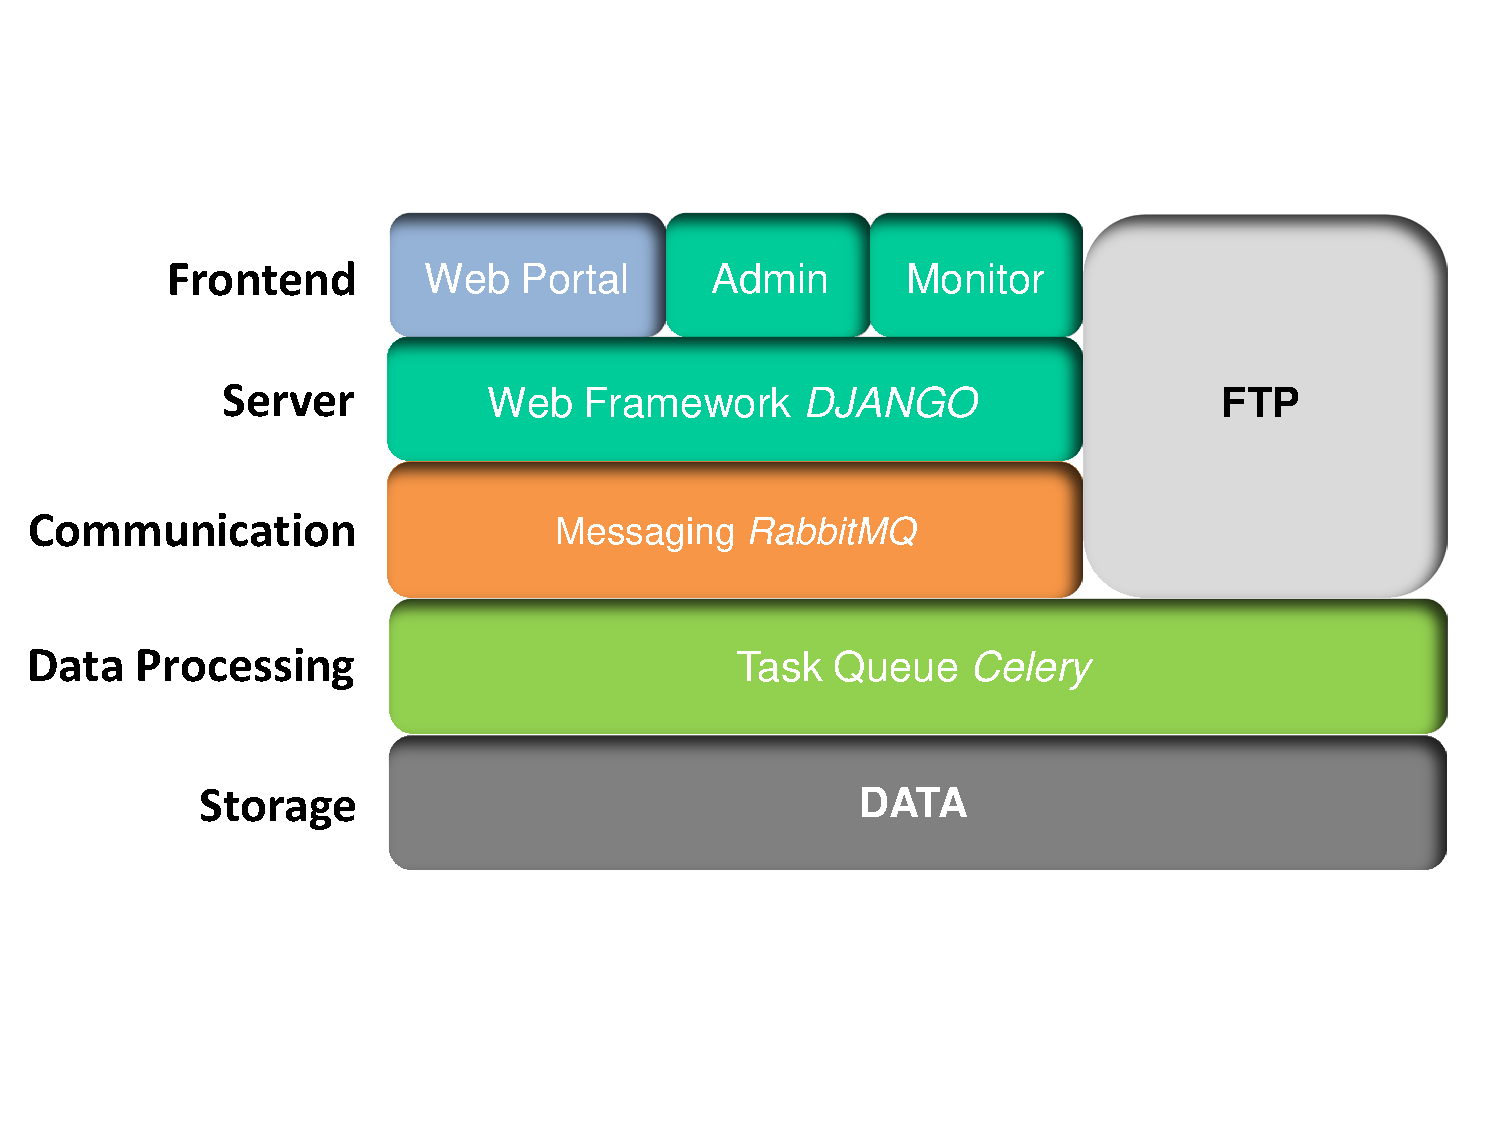
\includegraphics[height=0.35\textheight]{pics/KCDC-IT-Structure.pdf}
\end{frame}

\begin{frame}{KASCADE and TAIGA data rates}
\begin{minipage}[c]{0.52\textwidth}
% \small
  \begin{itemize}
    \item KASCADE:
    \begin{itemize}
      \item 450 000 000 events
      \item ~ 4 Tb of measured data
    \end{itemize}
    \vspace{1em}
    \item planned TAIGA rate: ~ 20 TB/year
    \begin{itemize}
      \item HiSCORE: ~ 18 TB/year
      \item IACT: 1.5 TB/year
      \item others: ~ 0.5 TB/year
    \end{itemize}
  \end{itemize}
\end{minipage}
\hfill
\begin{minipage}[c]{0.47\textwidth}
\vspace{-3.5em}
  \begin{itemize}
    \item current TAIGA rate: 
    \begin{itemize}
      \item ~ 50 Tb of raw data;
      \item ~ 8 TB/year of reconstructed data:
      \begin{itemize}
	\item HiSCORE: 6.4 TB/year
	\item IACT: 1 TB/year
	\item others: ~ 0.5 TB/year
      \end{itemize}
    \end{itemize}
  \end{itemize}
\end{minipage}

\end{frame}

\begin{frame}{Machine and deep learning opporutities}
 \begin{itemize}
  \item Search for anisotropies - Clasterisation;
  \item Distinguishing gamma/not gamma (distribution-based [$\beta$]) - Classification.
 \end{itemize}

\end{frame}
